\documentclass{article}

\usepackage{amsmath, graphicx, amssymb}

\title{Revis\~ao R\'apida de Processos At\^omicos e Nucleares}
\author{Rafael Lopes de S\'a}
\date{\today}

\begin{document}
\maketitle

\section{Efeito fotoel\'etrico}

\subsection{Resumo}

O efeito fotoel\'etrico consiste num el\'etron de um metal absorvendo um f\'oton de forma que esse el\'etron se torna livre:

\begin{equation}
\text{el\'etron ligado} + \text{f\'oton} \rightarrow \text{el\'etron livre}
\end{equation}



Se a energia do f\'oton absorvida pelo el\'etron for maior que a energia de liga\c c\~ao do el\'etron com a estrutura met\'alica, o el\'etron vai se tornar livre e pode formar uma corrente el\'etrica. Quase todo problema sobre efeito fotoel\'etrico se resolve usando conserva\c c\~ao de energia. Conceitualmente:

\begin{equation}
\begin{split}
(\text{energia do f\'oton}) &- (\text{energia gasta para liberar o f\'oton da estrutura met\'alica}) = \\
&(\text{energia cin\'etica do el\'etron livre}) + (\text{energia potencial do el\'etron livre})
\end{split}
\end{equation}

A energia gasta para liberar o f\'oton da estrutura met\'alica \'e algo complicado de se calcular e, em geral, representamos apenas por um s\'imbolo $\phi$ e pelo nome ``fun\c c\~ao trabalho''. \'E uma propriedade do metal e n\~ao do f\'oton.

A energia de um f\'oton \'e proporcional \`a sua freq\"u\^encia:
\begin{equation}
E_f = hf,
\end{equation}
onde $h$ \'e chamado de \textbf{constante de Planck}. A energia cin\'etica \'e dada pela f\'ormula familiar:
\begin{equation}
E_c = \frac{1}{2}mv^2.
\end{equation}
J\'a a energia potencial depende do seu sistema. Usualmente uma bateria pode ser conectada \`a celula fotoel\'etrica criando uma diferen\c ca de potencial. O el\'etron tem que ent\~ao ir de contra (se o polo positivo da bateria estiver ligado ao cotodo) ou a favor (de o polo negativo da bateria estiver ligado ao catodo) esse potencial e gastar\'a ou, respectivamente, receber\'a uma energia dada por:
\begin{equation}
E_p = Q_e\times V,
\end{equation}
onde $Q_e$ \'e a carga do el\'etron e V \'e a diferen\c ca de potencial da bateria. Colocando todos os conceitos juntos:
\begin{equation}\label{eq:energia}
hf - \phi = E_c + E_p = \frac{1}{2}mv^2 + Q_eV.
\end{equation}

Algumas coisas a se lembrar:
\begin{itemize}
\item No efeito fotoel\'etrico usual, cada f\'oton \'e absrovido por um el\'etron. Isso quer dizer que se a energia do f\'oton n\~ao for pelo menos a fun\c c\~ao trabalho $\phi$, n\~ao haver\'a corrente el\'etrica. No caso em que h\'a uma bateria tamb\'em, a energia do f\'oton tem que ser, pelo menos, a fun\c c\~ao trabalho mais a energia potencial provida pela bateria.
\item Se o el\'etron absorver um f\'oton de energia maior (isto \'e, de maior frequ\^encia), ele sair\'a com maior energia. Mas \textbf{n\~ao quer dizer que mais el\'etrons ser\~ao emitidos}.
\item Para emitir mais el\'etron, voc\^e precisa de mais f\'otons. Isso quer dizer uma luz incidente mais intensa.
\end{itemize}

\subsection{Constantes e unidades}

A unidade de energia no Sistema Internacional de unidades \'e o Joule. $1\,\text{J}$ \'e uma quantidade muito grande para efeitos at\^omicos e subat\^omicos. Uma unidade conveniente \'e o $\text{eV}$. 1 $\text{eV}$ \'e definido como a energia que 1 (um) el\'etron tem num potencial de 1 (um) Volt. Para converter para o SI, basta usar a carga do el\'etron:

\begin{itemize}
\item $1\,\text{eV} = 1.6\times 10^{-19}\text{J}$,
\item $1\,\text{J} = 1/(1.6\times 10^{-19})\,\text{eV} = 6.24\times 10^{18}\,\text{eV}$ ,
\end{itemize}
pela pr\'opria defini\c c\~ao de $\text{eV}$ a carga el\'etrica fundamental \'e escrita como $e = 1.6\times 10^{-19}\,\text{C} = 1\,\text{eV/V}$.

Algumas constantes:

\begin{itemize}
\item $h = 6.626\times 10^{-34}\,\text{J s} = 4.136\times 10^{-15}\,\text{eV s}$,
\item $c = 3\times 10^{8}\,\text{m/s}$.
\item $hc = 1240\,\text{eV nm}$
\end{itemize}
O valor de $hc$ \'e conveniente porque, muitas vezes, \'e dado o comprimento de onda ($\lambda$) do f\'oton em vez da freq\"u\^encia. Essas duas quantidades se relacionam por:

\begin{equation}
c = \lambda f,
\end{equation}
logo, a energia de um f\'oton com comprimento de onda $\lambda$ \'e dada por:
\begin{equation}
E = hf = \frac{hc}{\lambda}.
\end{equation}

Algumas vezes tamb\'em \'e conveniente usar $\text{eV/c}^2$ como unidade de massa e $eV/c$ como unidade de momento linear. Nessa unidade, a massa do el\'etron é dada por:
\begin{equation}
m_e = 511\, \text{keV/c}^2.
\end{equation}

\subsection{Um exemplo t\'ipico}

A figura abaixo representa o arranjo t\'ipico do efeito fotoel\'etrico:

\begin{figure}[h]
\centering
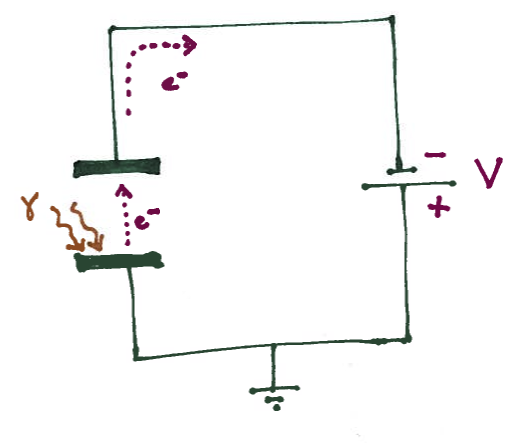
\includegraphics{circuito.png}
\caption{Arranjo t\'ipico do efeito fotoel\'etrico. Note que a luz indice sobre a placa inferior, chamada \textbf{anodo}, enquanto a placa superior, chamada \textbf{catodo}, coleta el\'etrons que conseguem se libertar do metal do anodo e est\~ao no v\'acuo entre as placas. Para mais detalhes veja texto.}
\end{figure}
A luz incide sobre a placa inferior. Se os f\'otons tiverem mais energia que a \textbf{fun\c c\~ao trabalho}, isto \'e, que a energia necess\'aria para liberar os el\'etrons da estrutura met\'alica, esse el\'etrons v\~ao escapar para o v\'acuo entre as placas, como representado pela seta pontilhada. Contudo, note que h\'a tamb\'em uma bateria no circuito. Essa bateria faz com que o fio na parte de cima esteja num potencial diferente do fio embaixo. Se assumirmos que o potencial do fio embaixo \'e 0, o potencial do fio de cima ser\'a negativo. Voc\^e pode dizer isso pela orienta\c c\~ao da baterial: veja que o terminal negativo (linha curta) est\'a ligada ao fio de cima.

Como el\'etrons s\~ao negativos e o potencial \'e negativo, os el\'etrons experimentam uma for\c ca contra seu movimento. Dito de outra forma, como tanta a carga do el\'etron quando o potencial el\'etrico \'e negativo, ent\~ao a energia potencial do fio em cima:

\begin{equation}
E_p = Q_E\times V > 0,
\end{equation}
\'e positiva. Num an\'alogo gravitacional, \'e como se houvesse uma montanha que os el\'etrons tem que subir e eles s\'o conseguem entrar no fio de cima se subirem essa montanha. Isto quer dizer que os el\'etrons tem que gastar essa energia potencial para conseguir se propagar no fio. Isso, claro, al\'em da energia gasta para se liberar da estrutura met\'alica (fun\c c\~ao trabalho). Desta forma, a energia cin\'etica do el\'etron \'e dada pela equ\c c\~ao \eqref{eq:energia}:
\begin{equation}
E_c = hf - \phi - Q_e\times V.
\end{equation}
A energia cin\'ética \'e um n\'umero maior ou igual a zero. Quando a energia cin\'etica dos el\'etrons \'e zero, isso quer dizer que n\~ao h\'a corrente el\'etrica (os el\'etrons n\~ao chegam no catodo). O potencial para o qual isso acontece \'e dado por:
\begin{equation}
0 = hf - \phi - Q_e\times V_{\text{max}}.
\end{equation}
Essa \'e uma maneira muito conveniente de se medir a fun\c c\~ao trabalho de um potencial. Dado que voc\^e sabe a freq\"u\^encia do f\'oton e o potencial da baterial em que a corrente cessa ($V_{\text{max}}$), a fun\c c\~ao taabalho pode ser encontrada resolvendo a equa\c c\~ao acima:
\begin{equation}
\phi = hf - Q_e\times V_{\text{max}}.
\end{equation}

\subsection{Sobre a energia cin\'etica dos el\'etrons}
Para entender a energia cin\'etica que os el\'etrons ter\~ao no circuito \'e importante primeiro entender a energia que eles tem enquanto est\~ao num s\'olido. Isso pode ser visto no diagrama da figura \ref{fig:bandas}. Sem a incid\^encia de luz, os el\'etrons com maior energia num metal estar\~ao na banda intermedi\'aria. Essa \'e a chamada banda de condu\c c\~ao. Isso quer dizer que eles podem se propagar livremente dentro do material (por isso que metais conduzem eletricidade), mas n\~ao podem escapar do material. A energia de el\'etrons livre \'e maior que el\'etrons de condu\c c\~ao e a diferen\c ca entre as duas bandas de energia \'e justamente a fun\c c\~ao trabalho que j\'a definimos acima.

\begin{figure}[ht]
\centering
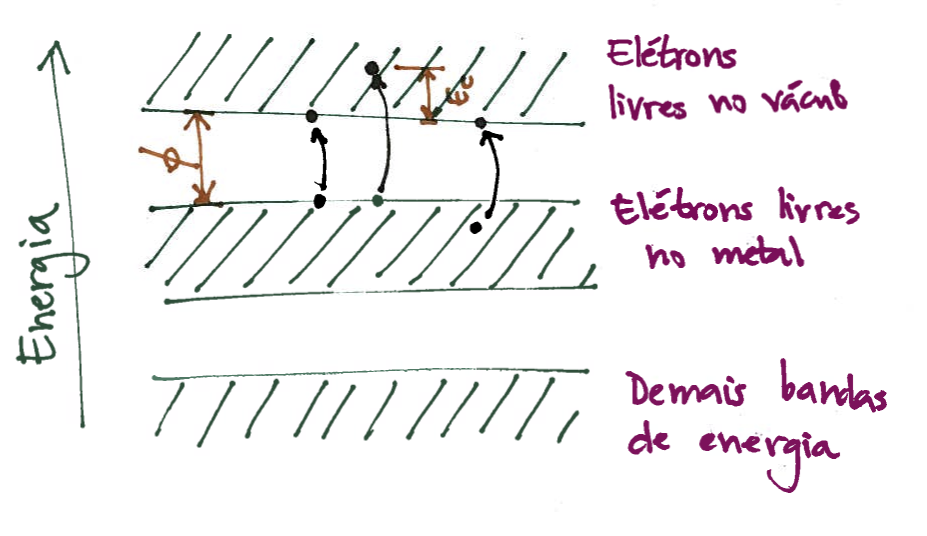
\includegraphics[width=0.9\textwidth]{bandas.png}
\caption{\label{fig:bandas}Estrutura de energia em bandas de um el\'etron num s\'olido. A figura mostra a chamada \textbf{banda de condu\c c\~ao}, na qual os el\'etrons podem se propagar livremente dentro do material e a diferen\c ca de energia $\phi$ para que os el\'etrons escapem do estrutura do material e possam se propagar livremente no v\'acuo fora do material. A diferen\c ca de energia entre essas duas bandas de energia \'e chamada \textbf{fun\c c\~ao trabalho} $\phi$.}
\end{figure}
Note que s\'olidos s\~ao essencialmente diferente de \'atomos livres. Em \'atomos livres (como num g\'as), os el\'etrons s\'o podem ter energias discretas bem definidas. Em s\'olidos eles podem ter \textbf{qualquer energia} em \textbf{bandas de energias}. Ent\~ao podemos imaginar diversas situa\c c\~oes distintas para como o efeito fotoel\'etrico ocorre no metal. Os tr\^es casos que quero discutir s\~ao representados pelas tr\^es setas escuras.

No primeiro caso (mais a esquerda), o el\'etron absorve um f\'oton que tem energia \textbf{exatamente} igual a fun\c c\~ao trabalho. Isso quer dizer que o el\'etron s\'o vai sair do material se ele tiver a maior energia poss\'ivel na banda de condu\c c\~ao. Se a energia dele fosse um poquinho menor, ele n\~ao escaparia. E, mesmo quando escapa, ele fica livre, mas parado, pois n\~ao sobra nenhuma energia como energia cin\'etica.

Nos dois outros casos o f\'oton tem mais energia que a fun\c c\~ao trabalho. Ent\~ao duas coisas podem acontecer. Esse f\'oton pode ser absorvido por um el\'etron na borda da banda de condu\c c\~ao, isto \'e, com a maior energia poss\'ivel dentro do material. Neste caso, o el\'etron se libera e ainda ter\'a uma energia cin\'etica $E_c$. Mas tamb\'em pode acontecer do f\'oton ser absrovido por um el\'etron com um pouco menos de energia (mais a direita na figura). Neste caso ele se liberar\'a, mas sua energia cin\'etica depois disso ser\'a zero.

A id\'eia que quero passar aqui \'e que a energia cin\'etica que escrevemos na f\'ormula \eqref{eq:energia}, n\~ao vai ser a energia cin\'etica de \textbf{todo} el\'etron liberado, mas sim a maior energia poss\'ivel. Alguns el\'etrons tinha uma energia menor dentro do material. Logo, algumas vezes voc\^e vai ver escrito:

\begin{equation}
E_c^{\text{max}} = hf - \phi - E_p.
\end{equation}

\section{Bremsstrahlung}

\subsection{Resumo}
O proceso de bremsstrahlung tem os seguintes estados iniciais e finais:

\begin{equation}
\text{el\'etron livre} \rightarrow \text{el\'etron livre} + \text{f\'oton}.
\end{equation}
A palavra bremsstrahlung vem do alem\~ao e significa, literalmente, energia de frenamento. Isso porque o el\'etron \'e desacelerado durante o processo. Em outras palavras, o el\'etron livre do estado final tem uma energia cin\'etica maior que a o el\'etron no estado final. A diferen\c ca entre as duas energias \'e a energia do f\'oton. Logo, a freq\"u\^encia, $f$, do f\'oton emitida \'e:

\begin{equation}\label{eq:energia2}
f = \frac{E_c(\text{el\'etron final})-E_c(\text{el\'etron inicial})}{h}
\end{equation}

Essa \'e uma das formas mais comuns de se produzir raio X. As m\'aquinas de raio X em hospitais, por exemplo, usam exatamente esse m\'etodo. Aqui estamos assumindo duas coisas:

\begin{enumerate}
\item O el\'etron perde toda sua energia cin\'etica.
\item Toda a energia \'e transferida para apenas um f\'oton.
\end{enumerate}
Ambas hip\'oteses n\~ao s\~ao necessiaramente verdade. O el\'etron perde sua energia interagindo com algum material, vamos supor que esse material \'e exposso o suficiente para parar o el\'etron. Isto \'e, o caso (1) acima n\~ao nos interessa aqui. No segundo caso, o el\'etron pode emitir diversos f\'otons tal que a soma de todas as energias emitidas \'e igual a sua energia inicial. Nesse caso cada f\'oton individual ter\'a uma frequ\"u\^encia (e, logo, energia) menor do que aquela escrita em \eqref{eq:energia2}.

\subsection{Em pequeno adendo sobre a f\'ormula para energia cin\'etica}

A f\'ormula da energia cin\'etica que vimos acima:
\begin{equation}
E_c = \frac{1}{2}m_ev^2,
\end{equation}
s\'o \'e v\'alida para el\'etrons com baixa energia. Se quisermos produzir f\'otons com alta energia atrav\'es de bremsstrahlung, ent\~ao precisamos a f\'ormula correta para energia cin\'etica. Alta energia quer dizer que a estamos falando de f\'otons com energia maior que a massa do el\'etron, isto \'e, $hf > 511\,\text{keV}$.

A f\'ormula exata a ser usada nesse caso \'e:
\begin{equation}
E_c = \frac{mc^{2}}{\sqrt{1-\frac{v^2}{c^2}}} - mc^2,
\end{equation}
onde o primeiro termo \'e a energia total do el\'etron e o segundo termo \'e a chamada energia de repouso. A rela\c c\~ao equivalente para o momento linear \'e:
\begin{equation}
p = \frac{mv}{\sqrt{1-\frac{v^2}{c^2}}}.
\end{equation}

\subsection{Espectro real\'istico de emissão de raio X}
Num processo de Bremsstrahlung real\'istico (e, por isso, pass\'ivel de ser similar aos problemas que voc\^e vai encontrar), o el\'etron \'e primeira acelerado por um potencial el\'etrico. Como vimos acima, a energia potencial cedida por uma diferen\c ca de potencial $V>0$ \'e $Q_e\times V$. Como a energia inicial do el\'etron (antes da acelera\c c\~ao) \'e zero, a final tamb\'em tamb\'em tem que ser zero, isto \'e:

\begin{equation}
0 = E_c(\text{final}) + E_p(\text{final}) = \frac{1}{2}mv^2 + Q_e\times V.
\end{equation}
Note que $Q_e$, a carga do el\'etron, \'e um n\'umero negativo, de forma que a equa\c c\~ao faz sentido. Depois que o el\'etron foi aceelarado por esse potencial el\'etrico, ele \'e frenado atrav\'es da intera\c c\~ao com um material. O espectro de emiss\~ao de raio X pode ser visto na figura \ref{fig:brem}.

\begin{figure}[ht]
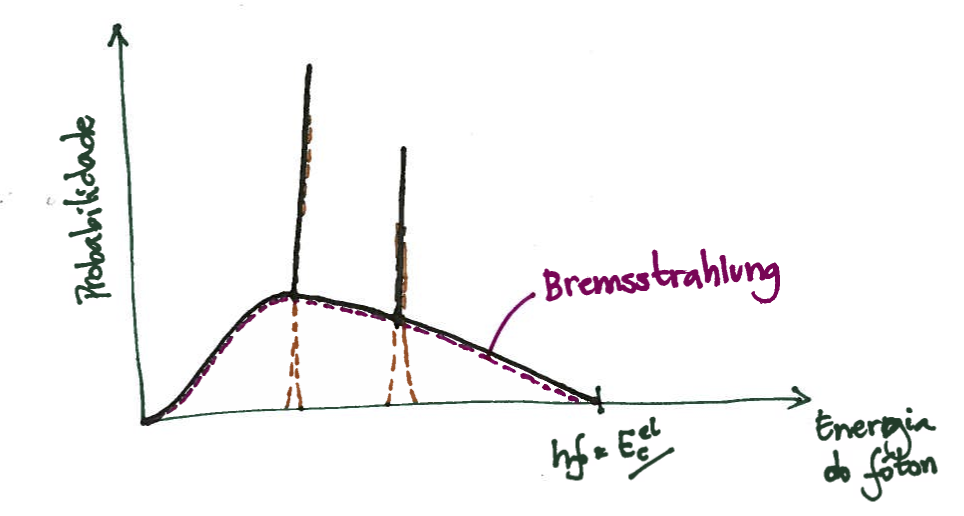
\includegraphics[width=0.9\textwidth]{brem.png}
\caption{\label{fig:brem}Espectro de energia do f\'oton emitido na desacelera\c c\~ao de um el\'etron ao interagir com um material. Note como a distribui\c c\~ao \'e a combina\c c\~ao de dois espectros distintos: um cont\'inuo (em roxo) e um discreto (em laranja). Vejo texto para explica\c c\~ao dos fen\^menos.}
\end{figure}
O espectro de energia dos f\'otons emitidos \'e a superposi\c c\~ao de dois espectros distintos. Um cont\'inuo, que corresponde \`a desacelera\c c\~ao do el\'etron devido \`a intera\c c\~ao com o campo el\'etrico e outro discreto, muito mais intenso mas em energias bem definidas. O espectro cont\'inuo \'e devido ao efeito de Bremsstrahlung descrito nessa se\c c\~ao. Veja na figura como a linha cont\'inua tem um ponto m\'aximo, que corresponde ao caso em que o el\'etron \'e completamente parado e toda sua energia \'e transferida a um \'unico f\'oton.

As linhas de emiss\~ao discretas correspondem a outro tipo de processo at\^omico, que estudaremos em seguida: emiss\~ao e absor\c c\~ao por \'atomos.

\section{Absor\c c\~ao e emiss\~ao de f\'otons por \'atomos}

Quando os \'atomos est\~ao livres, como num g\'as, o espectro de energia dos el\'etrons n\~ao \'e cont\'inuo, como no caso de el\'etrons livre, nem em bandas, como no caso de s\'olidos. As energias que os el\'etrons podem ocupar s\~ao discretas e cada n\'ivel de energia \'e chamado um \textbf{orbital at\^omico}. Calcular a energia de cada um desses orbitais \'e dif\'icil, a n\~ao ser no caso do hidrog\^enio, o que faremos mais a frente.

Como os n\'iveis s\~ao discretos, um el\'etron s\'o vai passar de um n\'ivel para outro se absorver um f\'oton que tem energia dada extamente pela diferen\c ca de energia dos dois orbitais. Esse processo chama\c c\~ao absor\c c\~ao (ou excita\c c\~ao) e \'e esquematicamente represtada por:

\begin{equation}
\text{el\'etron at\^omico ligado} + \text{f\'oton} \rightarrow \text{el\'etron at\^omico ligado}.
\end{equation}
Por conserva\c c\~ao de energia, a freq\"u\^encia de um f\'oton abosrvido entre orbitais com energia $E_1$ e $E_2$ tem que ser:

\begin{equation}
hf + E_1 = E_2.
\end{equation}
Esse processo \'e mostrado na figura \ref{fig:atom}. Em geral, escolhe-se a refer\^encia de energia para el\'etrons at\^omicos como a menor energia que el\'etrons livres podem ter. Essa refer\^encia \'e, como sempre arbitr\'aria (\'e equivalente a dizer qual \'e a ``altitude zero'', tanto faz, \'e apenas um ponto a partir do qual se mede), mas \'e conveniente j\'a que, desta forma, todo el\'etron livre ter\'a energia positiva e todo el\'etron ligado ao \'atomo num orbital ter\'a energia negativa. O processo de absor\c c\~ao \'e representado pela seta marrom apontando para cima. Um el\'etron, num n\'ivel de energia baixo $E_1$, aborve um f\'oton e faz uma transi\c c\~ao para um n\'ivel mais alto $E_2$. Isso s\'o ocorre se a energia do f\'oton for exatamente $E_2-E_1$.

\begin{figure}[ht]
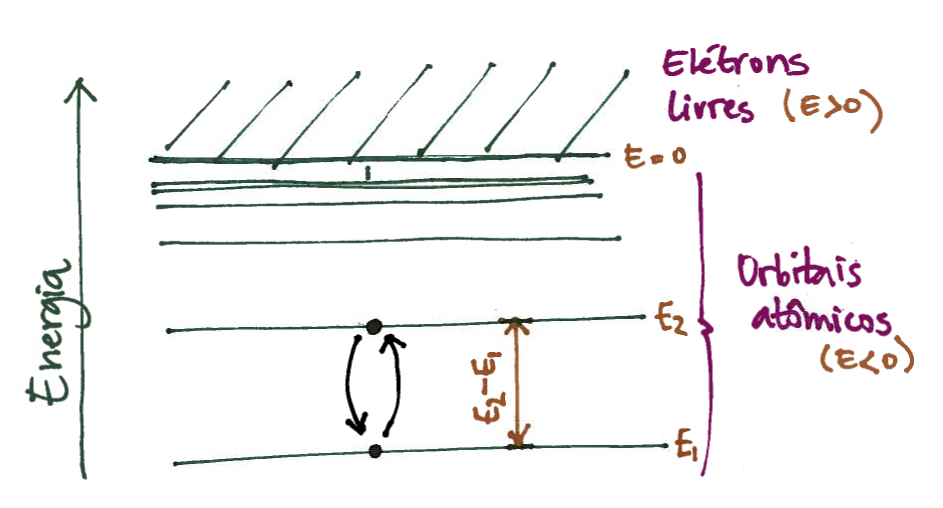
\includegraphics[width=0.9\textwidth]{atom.png}
\caption{\label{fig:atom}N\'iveis de energia de um el\'etron at\^omico. Os estados ligados possuem energia negativa ($E<0$) e existem apenas em n\'iveis de energia discretas. Os el\'etrons livre podem ter qualquer energia positiva $E>0$. Existem infinitos orbitais at\^omicos e a diferen\c ca de energia fica cada vez menor conforme os orbitais se aproximam de zero.}
\end{figure}

Um el\'etron num n\'ivel excitado, depois de um certo tempo, voltar\'a para o estado de menor energia, que \'e o \'unico est\'avel num \'atomo. Esse processo chama-se \textbf{emiss\~ao espont\^anea} e \'e esquematicamente dada pela seguinte rea\c c\~ao:


\begin{equation}
\text{el\'etron at\^omico ligado} \rightarrow \text{el\'etron at\^omico ligado} + \text{f\'oton}.
\end{equation}
Novamente usando conserva\c c\~ao de energia, podemos concluir que a energia do f\'oton ser\'a exatamente a diferen\c ca de energia entre os orbitais:

\begin{equation}
E_2 = E_1 + hf.
\end{equation}
A absor\c c\~ao e emiss\~ao espont\^anea s\~ao os processos pelos quais um \'atomo reage a incid\^encia de luz. Quando um f\'oton incide sobre um \'atomo, se ele tiver a energia correta para induzir uma transi\c c\~ao at\^omica, ele vai ser absorvido e, depois de um certo tempo, reemitido com a mesma frequ\^encia. Esse tempo que demora para ele ser reemitido \'e exatamente o que faz com que a luz, ao passar por um meio com \'atomos pare\c a mais lenta, apesar de cada f\'oton, individualmente, se propagar com a velocidade da luz $c$.

Existe um outro processo pelo qual um el\'etron pode ir de um n\'ivel de maior energia para um n\'ivel de menor energia, chamado de \textbf{emiss\~ao induzida}. Ele \'e esquematicamente dado por:

\begin{equation}
\text{el\'etron at\^omico ligado} + \text{f\'oton} \rightarrow \text{el\'etron at\^omico ligado} + 2\,\text{f\'otons}.
\end{equation}
Esse processo tamb\'em existe que a energia do f\'oton seja igual a diferen\c ca de energia dos orbitais at\^omicos envolvidos na transi\c c\~ao. Al\'em disso, os dois f\'otons no estado final ter\~ao a mesma frequ\^encia e mesma fase, isto \'e, o campo el\'etrico dos dois f\'otons oscilam exatamente da mesma forma (n\~ao necessariamente na mesma dire\c c\~ao, mas com mesma deped\^encia temporal).

Por fim, uma \'ultima possibilidade de intera\c c\~ao de f\'otons com \'atomos \'e o processo de \textbf{ioniza\c c\~ao}. Ele \'e esquematicamente dado por:
\begin{equation}
\text{el\'etron at\^omico ligado} + \text{f\'oton} \rightarrow \text{el\'etron livre}
\end{equation}
Como a energia de el\'etrons livres \'e continua, esse processo n\~ao exige que a energia do f\'oton seja exatamente igual a energia do orbital. Nesse caso, a energia do orbital \'e apenas a energi m\'inima para que o el\'etron se liberte. Qualquer energia acima disso tamb\'em ioniza o \'atomo e o excesso de energia se torna energia cin\'etica para o el\'etron.

\subsection{O \'atomo de hidrog\^enio}

O \'atomo de hidrog\^enio \'e o mais simples de todos os \'atomos pois possui apenas 1 (um) el\'etron. Nesse caso, os n\'iveis de energia podem ser calculados exatamente. Cada orbital do hidrg\^enio \'e classificado por um n\'umero natural $n\in \mathbb{N}$ e a energia desse n\'ivel \'e dada por:

\begin{equation}\label{eq:ryd}
E_n = -\frac{\text{Ry}}{n^2},
\end{equation}
onde $\text{Ry}$ \'e chamada cosntante de Rydberg e tem valor de $\text{Ry}=13.6\,\text{eV}$. Isso quer dizer que o n\'ivel de menor energia do \'atomo de hidrog\^enio \'e, para $n=1$, $-13.6\,\text{eV}$. Da\'i tamb\'em podemos concluir que qualquer f\'oton com mais de $-13.6\,\text{eV}$ \'e capaz de ionizar o hidrog\^enio. Um f\'oton de $13.6\,\text{eV}$ tem um comprimento de onda de $91\,\text{nm}$, ou seja, hidrog\^enio at\^omico \'e opaco para qualquer comprimento de onda menor que esse. A constante de Rydberg pode ser relacionada com constantes fundamentais da f\'isica da seguinte forma:

\begin{equation}
\text{Ry} = \frac{m_ee^4}{8\epsilon_0h^2},
\end{equation}
onde $m_e$ e $e$ s\~ao, respectivamente, a massa e carga do el\'etron, $\epsilon_0$ \'e a permissividade do v\'acuo e $h$ \'e a constante de Planck.

\subsection{\'Atomos de muitos el\'etrons e degeneresc\^encia dos orbitais}

\'Atomos com mais de um el\'etron possuem espectro muito mais complicado que o \'atomo de hidrog\^enio. N\~ao existem rela\c c\~oes simples como \eqref{eq:ryd} para os n\'iveis de energia e os orbitais podem ser calculados apenas aproximadamente. Alguns \'atomos, contudo, tem o espectro eletr\^onico (isto \'e, os n\'iveis de energias dos orbitais em que os el\'etrons podem estar) bem parecidos com o hidrog\^enio. 
\subsection{O processo de LASER}


\section{Decaimentos nucleares}

O processo de decaimento nuclear radioativo \'e um processo aleat\'orio, que acontece independentemente da hist\'oria passada do n\'ucleo e, em primeira aproxima\c c\~ao, da presen\c ca de outros n\'ucleos radioativos. Como o processo \'e aleat\'orio, tudo que podemos dizer \'e a probabilidade de um n\'ucleo decair num dado intervalo de tempo, mas n\~ao \'e poss\'ivel ter certeza se, ap\'os passagem de dado tempo o n\'ucleo ter\'a decaido ou n\~ao. A probabilidade de um n\'ucleo decair num certo intervalo de tempo $\Delta t$ \'e dado por:

\begin{equation}
P(\Delta t) = \lambda\times \Delta t.
\end{equation}
Note como a probabilidade n\~ao depende da hist\'oria anterior do n\'ucleo. N\~ao importa se um n\'ucleo radioativo \'e antigo ou velho, a probabilidade de decair num intervalo de tempo $\Delta t$ s\'o depende do intervalo e de $\lambda$.

Se tivermos uma cole\c c\~ao grande de n\'ucleos radioativos, como a probabilidade de cada n\'ucleo decair independete dos outros, em m\'edia, teremos $N \lambda \Delta t$ n\'ucleo deca\'idos ap\'os um intervalo de tempo $\Delta t$. Uma outra forma de dizer isso \'e que a velocidade de desaparecimento dos n\'ucleos \'e:

\begin{equation}\label{atividade}
\frac{\Delta N}{\Delta t} = -\lambda N,
\end{equation}
onde o signal negativo apenas indica que os n\'ucleos est\~ao desparecendo. A quantidade no lado direito da equ\c c\~ao \eqref{atividade}, $\lambda N$, chama-se \textbf{atividade} da amostra radioativa e indica quantos decaimentos, em m\'edia, se observa por unidade de tempo. Embora n\~ao seja imediato, podemos ``resolver'' a equa\c c\~ao acima para obter uma fun\c c\~ao da quantidade m\'edia de n\'ucleos que ainda se preservam sem decair depois de um tempo $t$:

\begin{equation}
N(t) = N(0)\times e^{-\lambda t}.
\end{equation}
A quantidade $N(0)$ denota quantos n\'ucleos sua amostra tem no in\'icio da observa\c c\~ao, isto \'e, no tempo $t=0$. Como essa rela\c c\~ao envolve a fun\c c\~ao exponencial, uma pequena revis\~ao \'e em ordem.

\subsection{Fun\c c\~oes exponenciais e logar\'itimicas}

A fun\c c\~ao exponencial:
\begin{equation}
\begin{split}
&f:\mathbb{R}\rightarrow \mathbb{R},\\
&f(x) = e^x,
\end{split}
\end{equation}
\'e definida para todos os reais e possui as seguintes propriedades:

\begin{enumerate}
\item $f(x+y)= e^{x+y} = e^x\times e^y = f(x)\times f(y)$
\item $f(x-y) = e^{x-y}= \frac{e^x}{e^y} = \frac{f(x)}{f(y)}$
\item $f(xy) = e^{xy} = (e^x)^y = f(x)^y$
\end{enumerate}

\end{document}

